\chapter{Le modifiche al SIMIOR}
Per accomodare le nuove funzionalità è stato necessario fare delle modifiche strutturali al SIMIOR, spaziando dal database a classi di gestione dei dati interne al front-end del progetto.
\section{Modifiche strutturali}\label{modifiche_strutturali}
Le modifiche fatte si possono raggruppare in tre punti:
\begin{itemize}
	\item Database
	\item Archivio Statico
	\item Front-End
\end{itemize}
\subsection{Il Database}
Il database è stato alterato per permettere l'inserimento dei valori MIC \footnote{Precedentemente il campo non esisteva e l'antibiogramma aveva solo la sensibilità per antibiotico}, è stata creata inoltre la tabella feedback per permettere di raccogliere segnalazioni o eventuali richieste da parte degli utenti.
La funzionalità di invio feedback è disponibile in ogni pagina del sito, accessibile tramite un click sul relativo tasto presente nella \textit{navbar} di fianco al nome utente, la sua attivazione genera un \textit{popup} con un campo di testo (di massimo 2048 caratteri) dove può essere inserito il messaggio. L'invio del feedback in questo modo, permette una raccolta più dettagliata delle informazioni utili al debug, quale la pagina su cui l'utente stava lavorando e i log del sistema.
\begin{figure}[h!]
	\centering
	
\includegraphics[width=.99\columnwidth]{images/navbar}
	\caption{\textit{Navbar con sezione feedback e nome utente}}
	\label{fig:feature_location}
\end{figure}
\newline
\subsection{L'Archivio statico}
Oltre al database che contiene i dati creati dagli utenti, il SIMIOR possiede dei dati "statici" che raramente richiedono una modifica, un esempio di questi dati sono i codici degli antibiotici definiti dal sistema ATC/DDD (Anatomical Therapeutic Chemical/Defined Daily Dose) o i codici dei microorganismi definiti dall'Istituto Superiore di Sanità.
Essi sono contenuti in un archivio, chiamato internamente \textit{SimiorSelect}, da cui provengono tutti i valori mostrati negli elementi \texttt{<select>} del front-end (da cui il nome), qualsiasi operazione che richieda un inserimento di dati non numerici fa riferimento a questo archivio, e l'estrazione referti non è da meno. Il difetto della precedente implementazione riguarda la struttura di queste informazioni, difatti i nomi dei microrganismi e degli antibiotici e i loro codici erano distribuiti su due liste differenti, richiedendo diverse righe di codice ogni qualvolta fosse necessario associare le due informazioni, contribuendo all'errore umano in caso di modifica delle stesse (per esempio l'aggiunta di ulteriori antibiotici).
Si è proceduto, quindi, alla conversione di questo archivio dal formato XML (più ostico da leggere umanamente) a formato JSON e all'utilizzo di mappe nei casi più adatti (nell'esempio fatto prima). Seguono due esempi dell'organizzazione dei dati, prima (XML):
\begin{lstlisting}[language=xml]
<antibiotico>
        <valore>Neomycin (oral)</valore>
        ...
        <valore>Nystatin</valore>
</antibiotico>
 <cod_antibiotico>
        <valore>A07AA01</valore>
        ...
        <valore>A07AA02</valore>
 </cod_antibiotico>
\end{lstlisting}
e dopo la conversione (JSON):
\begin{lstlisting}[language=json]
  "antibiotici": {
        "A07AA01": "Neomicina (orale)",
         ...,
        "A07AA02": "Nistatina",
 }
\end{lstlisting}
E' evidente la maggior semplicità (e leggibilità) della struttura utilizzata, che mostra i suoi effetti anche nelle prestazioni, infatti l'utilizzo di mappe Chiave-Valore permette un accesso più rapido rispetto a un doppio scorrimento della lista, difatti la complessità (in termini di tempo) della ricerca lineare è $O(N)$, visto lo scorrimento di due liste diventa $2*O(N)$, l'accesso tramite mappa viene fatto calcolando l'hash che è sempre eseguito in tempo costante $O(1)$.
Queste modifiche si rivelano particolarmente utili in tutti quei casi dove è necessario recuperare i codici degli antibiotici o dei microrganismi, come nel caso dell'inserimento di un antibiogramma (sia tramite la nuova funzionalità sia manualmente) dove è necessario convertire un nome \textit{human-friendly} in una stringa identificativa univoca.
Oltre alla conversione è stata effettuata anche la traduzione di determinati valori, difatti i referti indicano gli antibiotici e i microrganismi in italiano, mentre i dati dell'archivio derivano dal sistema internazionale di classificazione, pertanto sono indicati in lingua inglese. Esistono dei casi particolari in cui alcuni antibiotici indicati nei PDF hanno un nome alternativo, spesso il nome scientifico, che viene gestito con l'aggiunta della corretta alternativa fra parentesi vicino al nome principale (es: la \textit{Benzilpenicillina benzatinica} comunemente conosciuta come \textit{Benzatina penicillina G} sarà indicata come un solo nome cosi strutturato: \textit{"Benzilpenicillina benzatinica (benzatina penicillina G)"})
\newpage
\section{Front-End}
L'utente può utilizzare la funzionalità recandosi nella sezione \textit{infezione, contaminazione o colonizzazione} di un qualsiasi ricovero, dove troverà una scheda contenente l'essenziale per poter allegare un referto e procedere con il caricamento.
Ogni sezione è stata progettata per essere semplice e analoga ad altre parti del progetto per evitare confusione da parte dell'utilizzatore finale, che è già abituato ai meccanismi del sistema. Infatti, la schermata dei risultati ha lo stesso aspetto dell'inserimento manuale dell'antibiogramma (una funzione di base del SIMIOR) con qualche aggiunta resa necessaria.
\subsection{Collocazione della funzionalità}
\begin{figure}[h!]
	\centering
	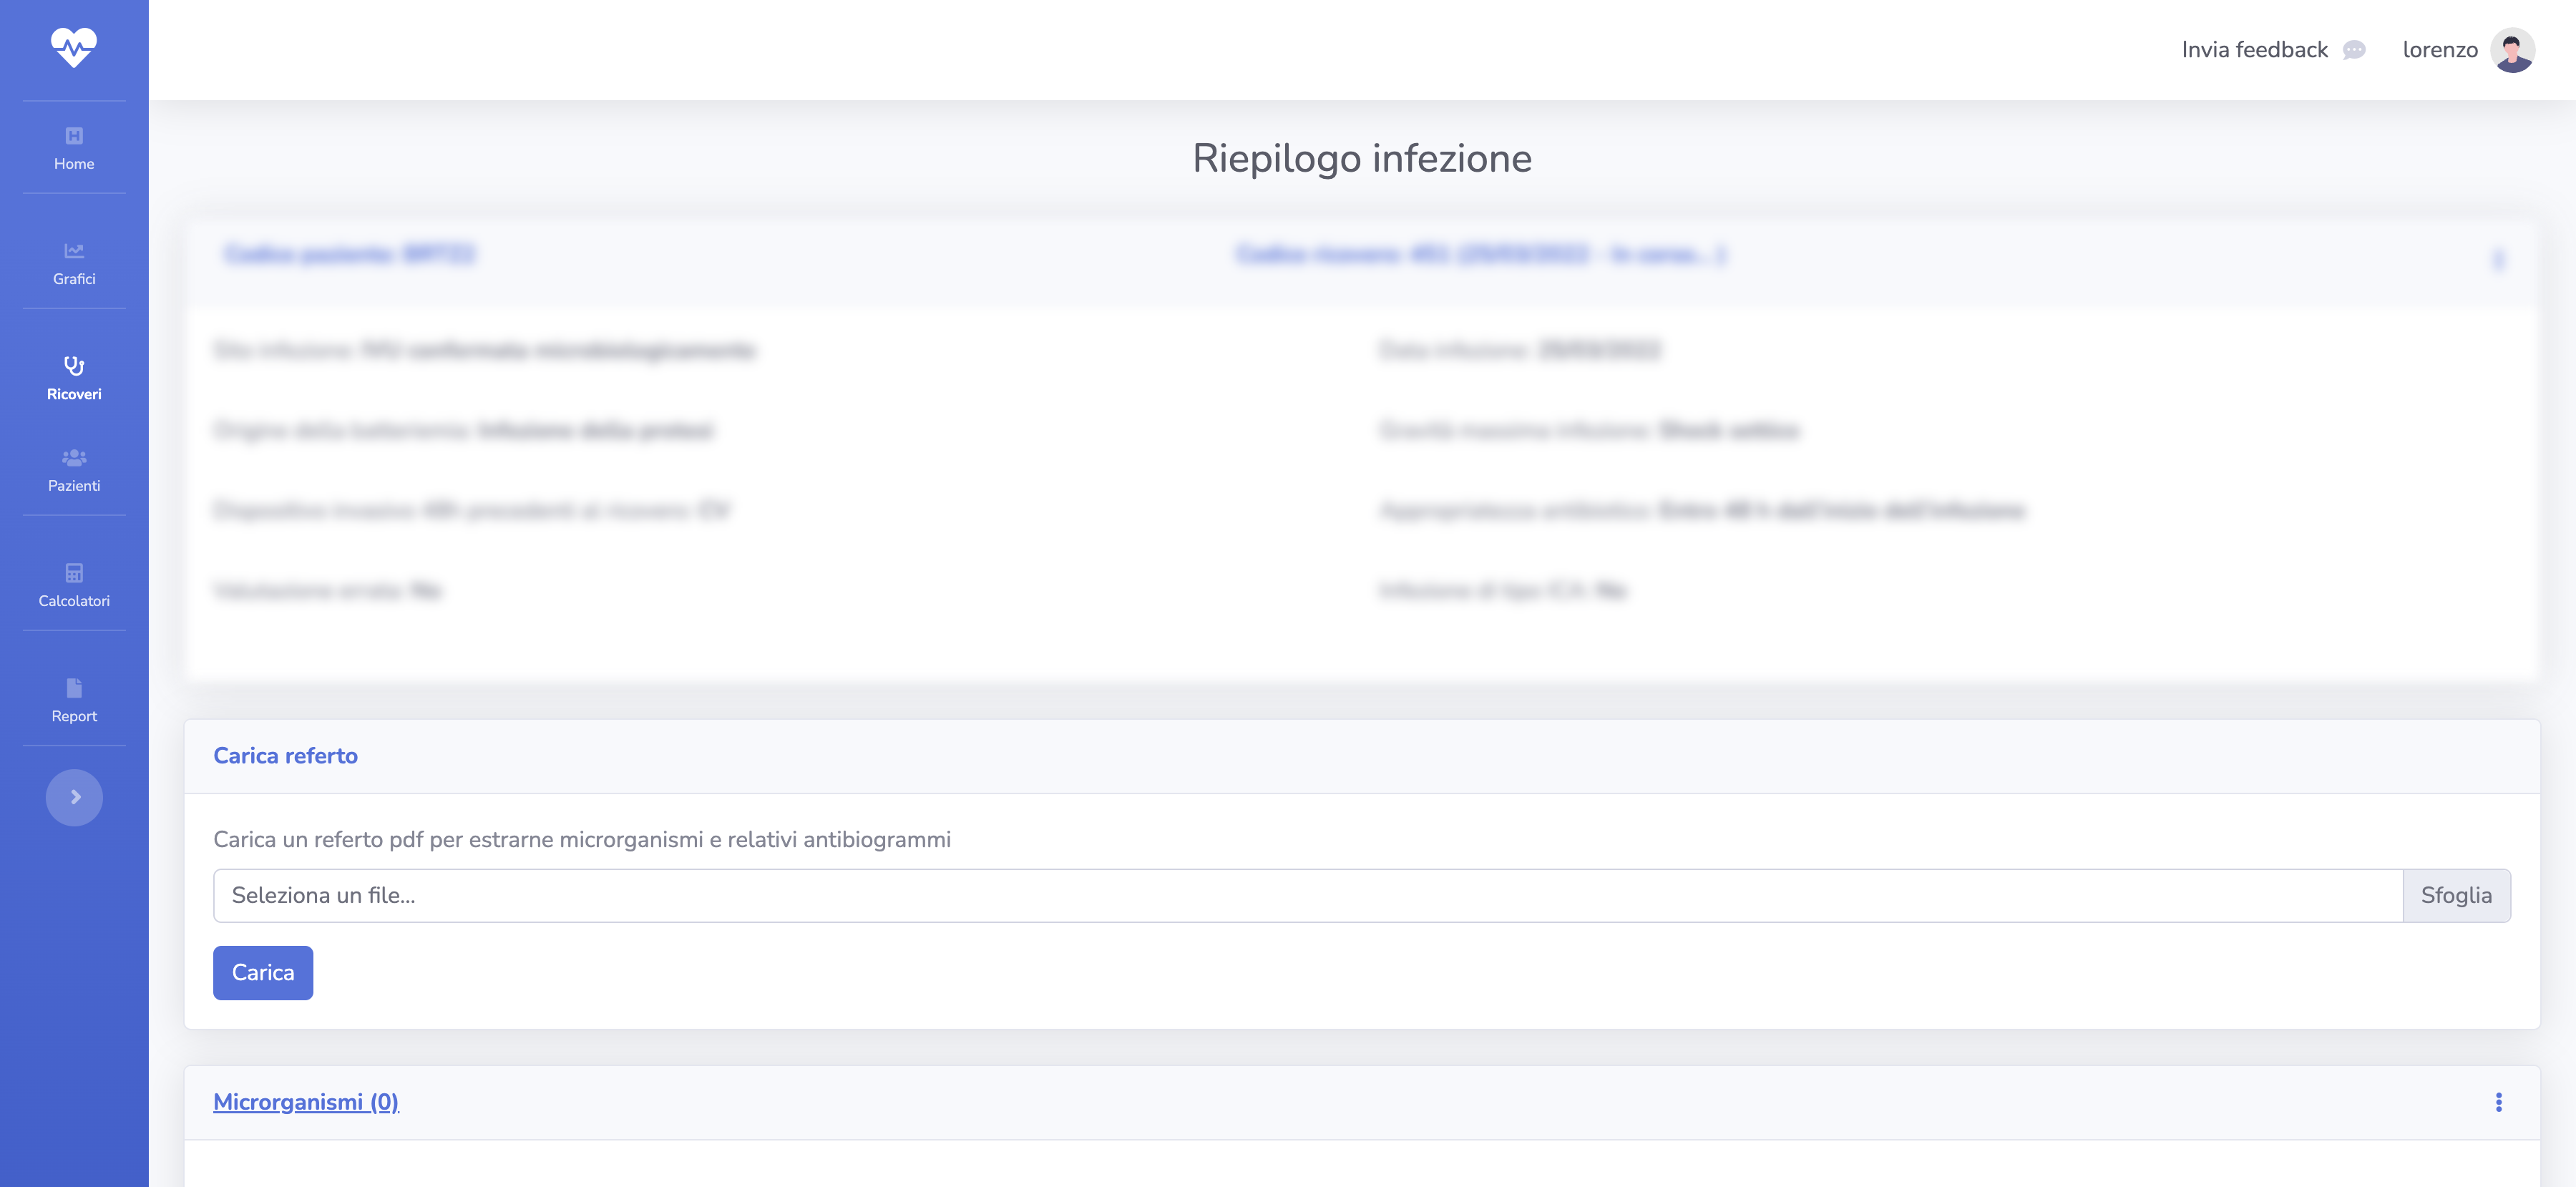
\includegraphics[width=.99\columnwidth]{images/feature_location.png}
	\caption{\textit{Scheda upload documento}}
	\label{fig:feature_location}
\end{figure}
La pressione del tasto \textit{"Sfoglia"} aprirà una schermata di dialogo gestita dal sistema che permetterà di selezionare il file determinato. Fatto questo l'utente procede alla pressione del tasto \textit{Carica} che lo porterà a una seconda pagina dove verranno mostrati i risultati dell'estrazione.
\newpage
\subsection{La schermata dei risultati}
Una volta eseguita da parte del back-end l'elaborazione del documento, i risultati vengono mostrati all'utente, il quale avrà la possibilità di apportare modifiche o confermare i dati estratti.
Nella sezione superiore della pagina delle schede mostreranno un breve riepilogo, informando l'utilizzatore quali microrganismi hanno un antibiogramma valido ed eventuali microrganismi e antibiotici sconosciuti al sistema (quindi non presente nell'archivio statico, vedi sezione \ref{modifiche_strutturali}).
\begin{figure}[h!]
	\centering
	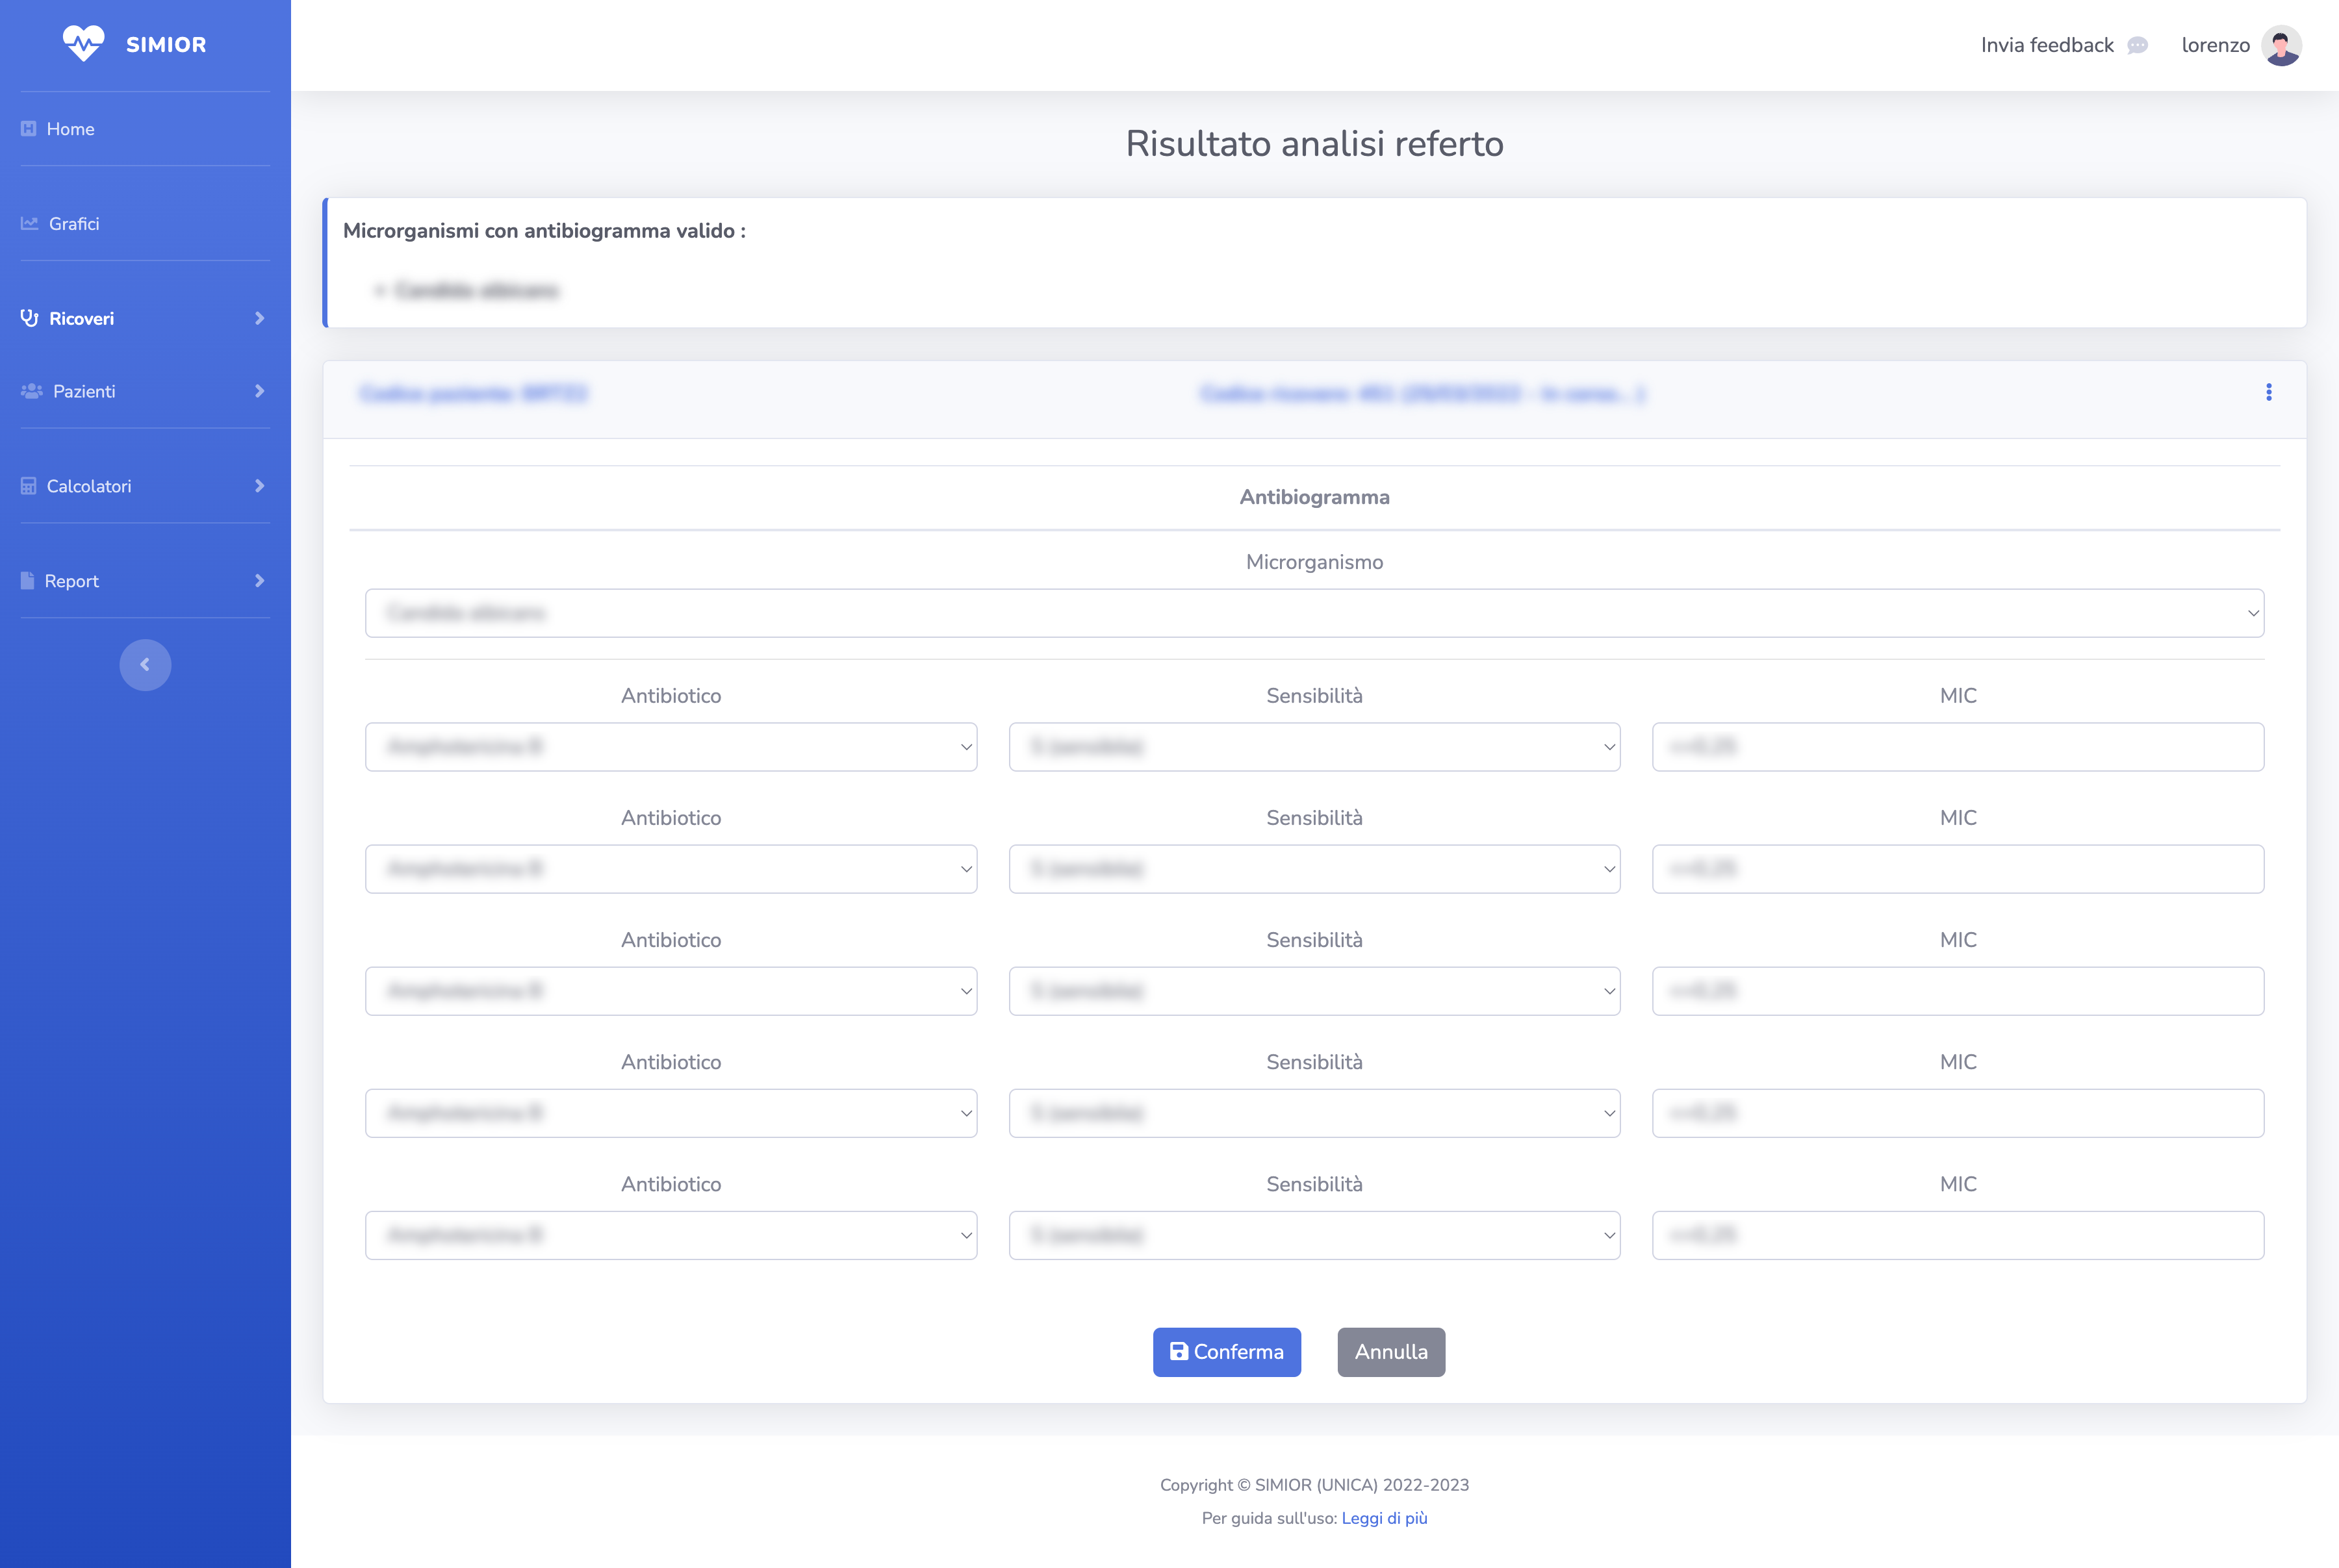
\includegraphics[width=.99\columnwidth]{images/extraction_result.png}
	\caption{\textit{Risultati estrazione}}
	\label{fig:extraction_result}
\end{figure}
\newline
Se un microrganismo non è presente nel sistema non è possibile inserire neanche il relativo antibiogramma perché non sarebbe poi possibile farvi riferimento successivamente.
\begin{figure}[h!]
	\centering
	
\includegraphics[width=.99\columnwidth]{images/static_missing.png}
	\caption{\textit{Microrganismo sconosciuto}}
	\label{fig:missing_micro}
\end{figure}
\newline
Allo stesso modo vengono segnalati eventuali antibiotici sconosciuti, ma a differenza del caso precedente, è comunque possibile procedere con l'inserimento dell'antibiogramma che verrà mostrato mancante dell'antibiotico relativo.
\begin{figure}[h!]
	\centering
	
\includegraphics[width=.99\columnwidth]{images/static_missing_antib.png}
	\caption{\textit{Antibiotico sconosciuto}}
	\label{fig:missing_anti}
\end{figure}
\newpage
In caso non tutti i dati siano estratti correttamente è possibile aggiungere o togliere manualmente informazioni, le opzioni di aggiunta sono disponibili nel menù \textit{drop-down} posizionato in alto a destra nella scheda contenente la tabella.
Per modificare un valore errato è sufficiente scegliere un'alternativa nella relativa lista, mentre per eliminare un valore (antibiotico o microrganismo) si seleziona l'elemento vuoto nella lista (indicato con un trattino), l'eliminazione ha un effetto 
"a cascata" che segue la seguente gerarchia: microrganismo -> antibiotico -> MIC e sensibilità, quindi l'eliminazione dell'antibiotico elimina l'intera riga mentre l'eliminazione del microrganismo elimina l'intero antibiogramma associato
\begin{figure}[h!]
	\centering
	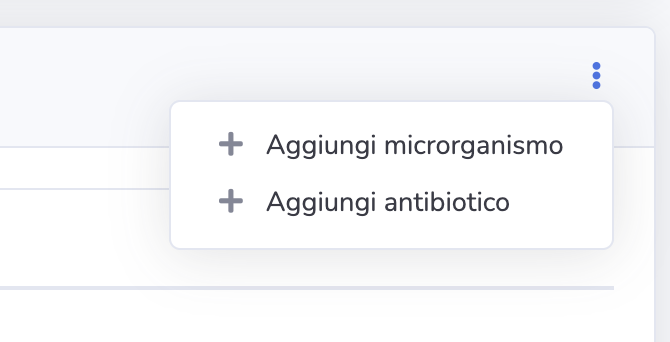
\includegraphics[width=.99\columnwidth]{images/new_object.png}
	\caption{\textit{Drop-down con le opzioni}}
	\label{fig:new_object}
\end{figure}
\newpage
Nel caso di più antibiogrammi estratti viene generata una pagina per ognuno di essi
\begin{figure}[h!]
	\centering
	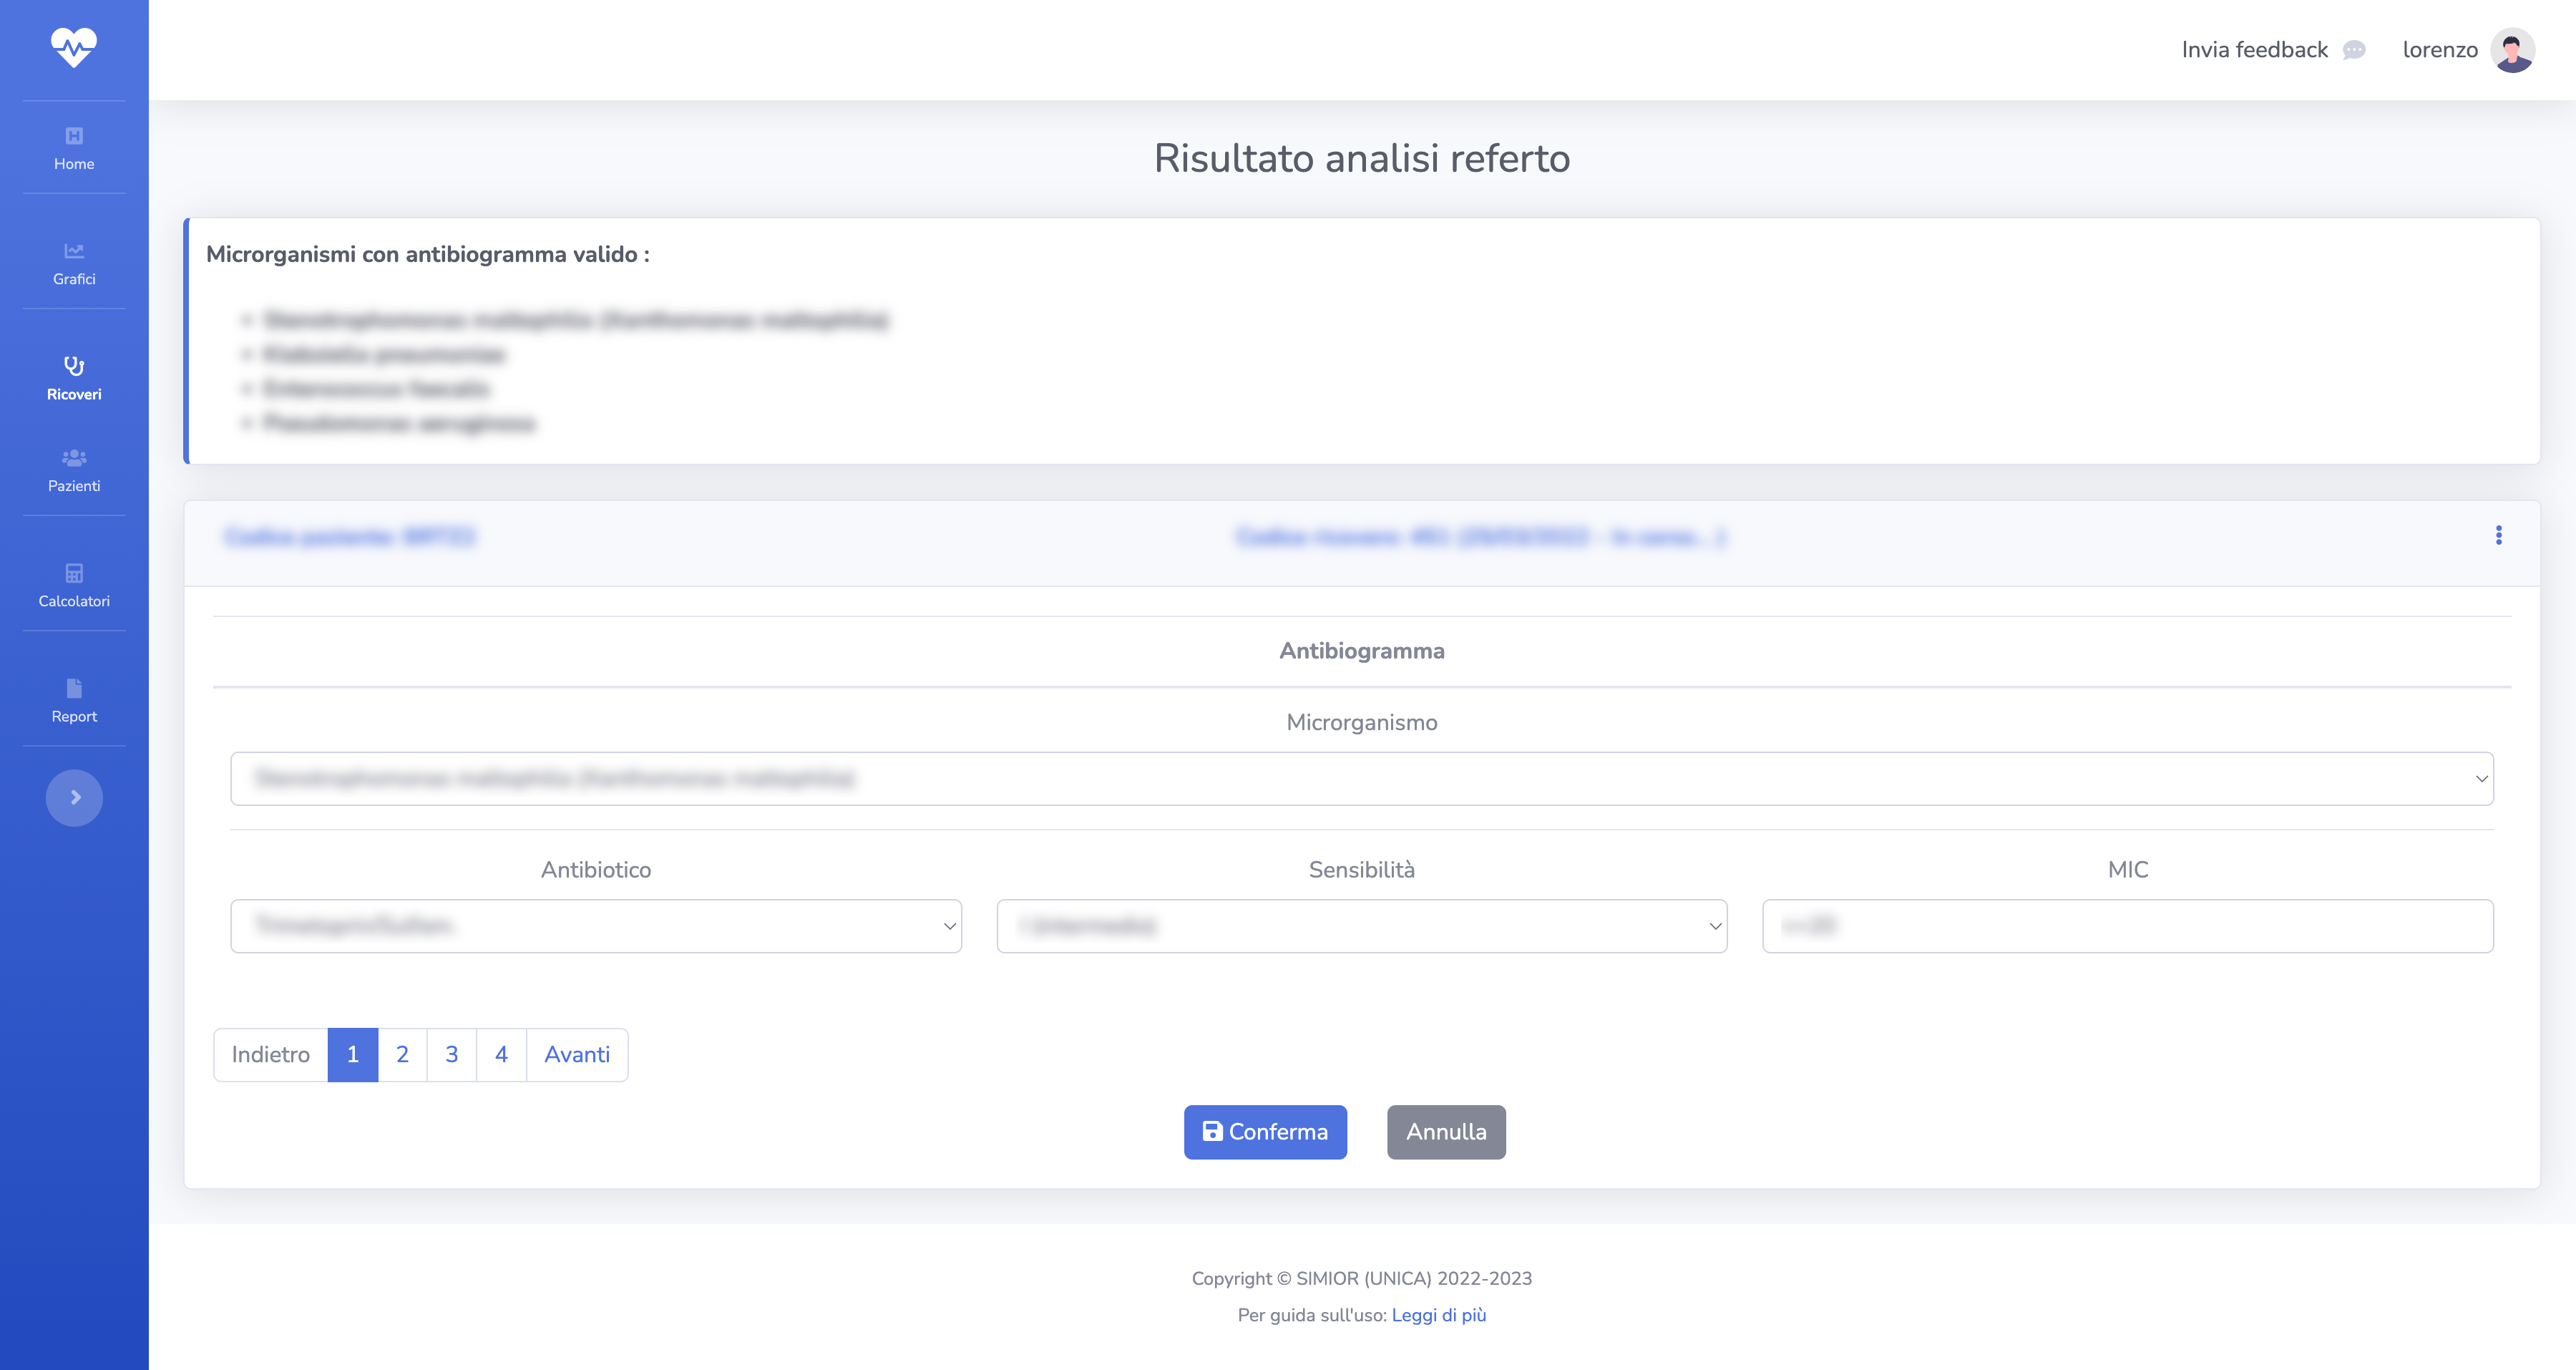
\includegraphics[width=.99\columnwidth]{images/result_multi.png}
	\caption{\textit{Risultato estrazione di quattro antibiogrammi}}
	\label{fig:result_multi}
\end{figure}
\newpage
\subsection{Conferma dei risultati}
Una volta apportate le modifiche ritenute opportune, l'utente conferma i dati col relativo tasto, e un messaggio indicherà il risultato dell'inserimento
\begin{figure}[h!]
	\centering
	
\includegraphics[width=.99\columnwidth]{images/confirm.png}
	\caption{\textit{Schermata di successo di inserimento}}
	\label{fig:confirm_success}
\end{figure}
\newline
Se il referto non contiene alcuna informazione valida (come mostrato nella figura \ref{fig:content_senza}) viene mostrato direttamente un messaggio di avviso senza possibilità di inserimento, in caso si deve procedere con un inserimento manuale (disponibile nella pagina di riepilogo)
\begin{figure}[h!]
	\centering
	
\includegraphics[width=.99\columnwidth]{images/no_table.png}
	\caption{\textit{Messaggio di informazione}}
	\label{fig:info_no_table}
\end{figure}


